\documentclass[paper=letter, fontsize=14pt]{scrartcl} 


\usepackage[utf8]{inputenc}
\usepackage{color}
\usepackage{graphicx}
\usepackage{epsfig}
\usepackage{multirow}
\usepackage{colortbl}
\usepackage[table]{xcolor}
\usepackage{fancyhdr}
\usepackage{graphicx}
\usepackage{graphicx}
\usepackage{verbatim}
\usepackage{pictex}  
\usepackage{multimedia}
\usepackage{listings}
\usepackage{vmargin}
\usepackage{xcolor,colortbl}
\usepackage[spanish]{babel} % language/hyphenation
\usepackage{amsmath,amsfonts,amsthm} % Math packages
\usepackage{amsbsy}
\usepackage{amssymb}
\usepackage{fancyvrb}
\usepackage{sectsty} % Allows customizing section commands
\allsectionsfont{\centering \normalfont\scshape} % Make all sections centered, the default font and small caps

\usepackage{fancyhdr} % Custom headers and footers
\pagestyle{fancyplain} % Makes all pages in the document conform to the custom headers and footers
\fancyhead{} % No page header - if you want one, create it in the same way as the footers below
\fancyfoot[L]{} % Empty left footer
\fancyfoot[C]{} % Empty center footer
\fancyfoot[R]{\thepage} % Page numbering for right footer
\renewcommand{\headrulewidth}{0pt} % Remove header underlines
\renewcommand{\footrulewidth}{0pt} % Remove footer underlines
\setlength{\headheight}{13.6pt} % Customize the height of the header

\numberwithin{equation}{section} % Number equations within sections (i.e. 1.1, 1.2, 2.1, 2.2 instead of 1, 2, 3, 4)
\numberwithin{figure}{section} % Number figures within sections (i.e. 1.1, 1.2, 2.1, 2.2 instead of 1, 2, 3, 4)
\numberwithin{table}{section} % Number tables within sections (i.e. 1.1, 1.2, 2.1, 2.2 instead of 1, 2, 3, 4)
\setpapersize{A4}
\setmargins{2.5cm}       % margen izquierdo
{2.4cm}                        % margen superior
{16.5cm}                      % anchura del texto
{23.42cm}                    % altura del texto
{10pt}                           % altura de los encabezados
{1cm}                           % espacio entre el texto y los encabezados
{0pt}                             % altura del pie de página
{2cm}                           % espacio entre el texto y el pie de página

\setlength\parindent{0pt} % Removes all indentation from paragraphs - comment this line for an assignment with lots of text

\newcommand{\horrule}[1]{\rule{\linewidth}{#1}} % Create horizontal rule command with 1 argument of height

\title{	
\normalfont \normalsize 
\textsc{Centro de Investigaci\'on en Matem\'aticas (CIMAT). Unidad Monterrey} 
\\ [25pt] 
\horrule{0.5pt} \\[0.4cm] % Thin top horizontal rule
\huge \textbf{Distribución de Wishart y Marchenko-Pastur}\\ 
\horrule{2pt} \\[0.5cm] % Thick bottom horizontal rule
}

\author{Ricardo Cruz} % Your name

\date{\normalsize\today} % Today's date or a custom date


\rhead{\begin{picture}(0,0) \put(-56.7,-50){
\includegraphics[width=20mm]{cimat.png}} \end{picture}}
\renewcommand{\headrulewidth}{0.5pt}

\pagestyle{fancy}

\begin{document}
\lstdefinestyle{customc}{
  belowcaptionskip=1\baselineskip,
  basicstyle=\footnotesize, 
  frame=lrtb,
  breaklines=true,
  %frame=L,
  %xleftmargin=\parindent,
  language=C,
  showstringspaces=false,
  basicstyle=\footnotesize\ttfamily,
  keywordstyle=\bfseries\color{green!40!black},
  commentstyle=\itshape\color{red!40!black},
  identifierstyle=\color{blue},
  stringstyle=\color{purple},
}

\lstset{breakatwhitespace=true,
  basicstyle=\footnotesize, 
  commentstyle=\color{green},
  keywordstyle=\color{blue},
  stringstyle=\color{purple},
  language=C++,
  columns=fullflexible,
  keepspaces=true,
  breaklines=true,
  tabsize=3, 
  showstringspaces=false,
  extendedchars=true}

\lstset{ %
  language=R,    
  basicstyle=\footnotesize, 
  numbers=left,             
  numberstyle=\tiny\color{gray}, 
  stepnumber=1,              
  numbersep=5pt,             
  backgroundcolor=\color{white},
  showspaces=false,             
  showstringspaces=false,       
  showtabs=false,               
  frame=single,                 
  rulecolor=\color{black},      
  tabsize=2,                  
  captionpos=b,               
  breaklines=true,            
  breakatwhitespace=false,    
  title=\lstname,             
  keywordstyle=\color{blue},  
  commentstyle=\color{dkgreen},
  stringstyle=\color{mauve},   
  escapeinside={\%*}{*)},      
  morekeywords={*,...}         
} 


\maketitle % Print the title


\pagebreak


Al realizar el proceso de componentes principales, una de las tareas más importantes es determinar el número de componentes que se considerarán. Usualmente se optar por elegir esta cantidad por medio de un screeplot o tomar los primeros valores propios que acumulen el 80 o 90\% de la varianza.\\

Esto se puede ejemplificar con para la matriz de covarianzas gaussiana. Sea $Z$ una matriz de $p\times n$, cuyas entradas se distribuyen normal estandar y $D$ una matriz diagonal de dimensión $p\times p$. Sea $X=DZ$, entonces, $XX'$ sigue una distribución Wishart con parámetros $n$ y $D^2$. Sea $S=XX'/n$ la matriz de covarianza muestral, se obtienen los valores propios de esta matriz, los cuales contienen la varianza explicada por la respectiva componente.\\

Tomando $p=30,n=\lbrace 30,300\rbrace D^2=diag(12,11,10,9,8,7,3,3,3,\hdots ,3)$, los valores propios ordenados para $n=30$ se muestran en la figura 1, mientras que la figura 2 los muestra para $n=300$\\

\begin{figure}[h]
  \centering
  \begin{minipage}[b]{0.4\textwidth}
    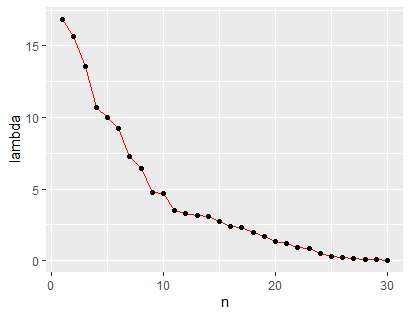
\includegraphics[width=\textwidth]{i1.png}
    \caption{n=30.}
  \end{minipage}
  \hfill
  \begin{minipage}[b]{0.4\textwidth}
    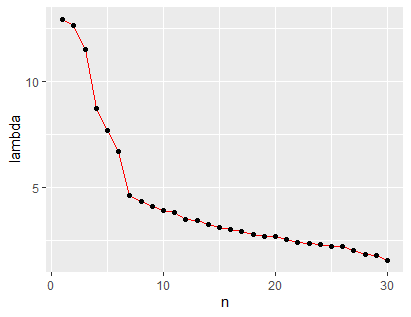
\includegraphics[width=\textwidth]{i2.png}
    \caption{n=300.}
  \end{minipage}
\end{figure}

Tomando el criterio del 80\%, se consideran 12 y 18 componentes para $n=30$ y $n=300$ respectivamente.

Para $n=300$ simulamos vía Montecarlo los 30 valores propios de la matriz $S$. Considerando 1000 simulaciones, se tiene la  densidad mostrada en la figura 3:\\

\begin{figure}[h]
\centering
	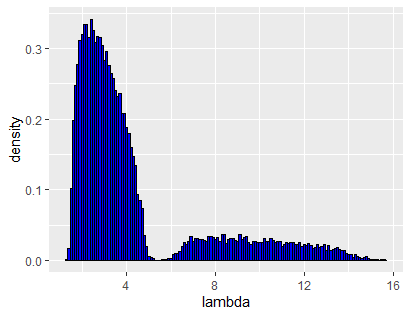
\includegraphics[scale=.75]{i3.png}
	\caption{densidad de las simulaciones de los eigenvalores.}
\end{figure}

Cuando $n,p$ son lo suficientemente grandes $n>p$, entonces $\dfrac{p}{n}\in(0,1)$, entonces los valores propios de la matriz que sigue la distribución Wishart tienen una densidad espectral dada por:
$$\rho(\lambda)=\dfrac{\sqrt{(\lambda_{max}-\lambda)(\lambda-\lambda_{min})}}{2*\pi*c*\lambda}$$
Donde $\lambda_{max}=(1+\sqrt{c})^2$ y $\lambda_{min}=(1-\sqrt{c})^2$. A esta densidad se le conoce como la ley de Marchenko-Pastur\\

Para el ejemplo que se ha manejado, ($n=300$) la figura 4 muestra la densidad vía la ley de Marchenko-Pastur y la figura 5 muestra las dos distribuciones hasta ahora generadas.\\


\begin{figure}[h]
  \centering
  \begin{minipage}[b]{0.4\textwidth}
    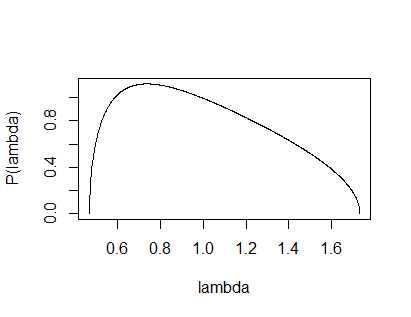
\includegraphics[width=\textwidth]{i4.png}
    \caption{MarchenkO-Pastur.}
  \end{minipage}
  \hfill
  \begin{minipage}[b]{0.4\textwidth}
    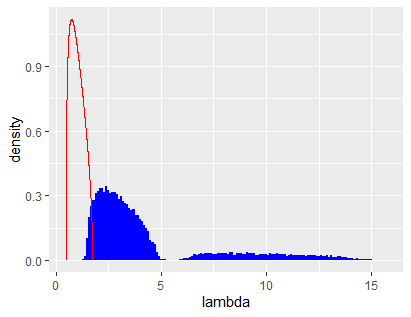
\includegraphics[width=\textwidth]{i5.png}
    \caption{Distribuciones-}
  \end{minipage}
\end{figure}

La ley de Marchenko-Pastur sugiere que los valores propios significativos (de los cuales se considerará la componente principal) son aquellos que son mayores al valor de $\lambda_{max}$.\\

Aplicando esta metodología, para $n=30$ se tomarían 10 componentes, mientras que para $n=300$ se toman 28 componentes. En ambos casos, se difiere de lo planteado originalemente por el screeplot o el critério del 80\%\\
\\


Ahora, para la matriz de correlación, las entradas que no se encuentran en la diagonal se distribuyen con media 0 y varianza $1/n$, por lo tanto, a medida que el tamaño de la muestra $n$ aumenta, el valor de dicha entrada es 0 con mayor seguridad, puesto que la varianza se aproxima a 0 a medida que $n$ crece y su media no se modificia.\\

Considerando una matriz aleatoria con $p=40$ y $n=\lbrace10,1000\rbrace$, las figuras 6 y 7 muestran los mapas de calor para las matrices de correlaciones con $n$ igual a 10 y 1000 respectivamente.

\begin{figure}[h]
  \centering
  \begin{minipage}[b]{0.4\textwidth}
    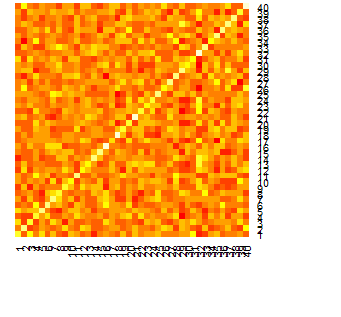
\includegraphics[width=\textwidth]{i6.png}
    \caption{n=10}
  \end{minipage}
  \hfill
  \begin{minipage}[b]{0.4\textwidth}
    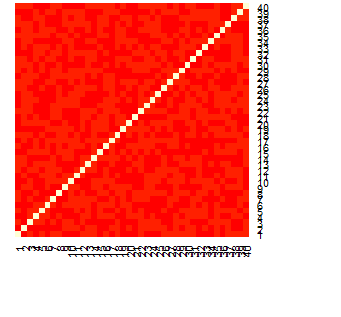
\includegraphics[width=\textwidth]{i7.png}
    \caption{n=1000}
  \end{minipage}
\end{figure}

Simulando 1000 veces la matriz de correlaciones, se puede obtener la media y desviación de cada entrada para los dos casos planteados para $n$.\\

Para $n=10$ las entradas de la diagonal tienen una media al rededor de 1 y su desviación es aproximadamente .4. Para los elementos que no están en la diagonal, la media es aproximadamente 0.04 y desviación de .3\\

Para $n=1000$ las entradas en la diagonal tienen media 1 y desviación aproximada de .04. Para los elementos en la diagonal, la media es aproximadamente 0, variando a partir de la cuarta posición después del punto y su desviación es aproximadamente .03.\\

Es por eso que el primer mapa de calor presenta mayor variación y el segundo solo dos colores, 1 en la diagonal y 0 en el resto de las entradas. Este efecto se conoce como \emph{noise dressing}, el cual depende del tamaño de la muestra.

\end{document}
